\documentclass[border=10pt]{standalone}
\usepackage{pgfplots}
\pgfplotsset{compat=1.18}
\begin{document}
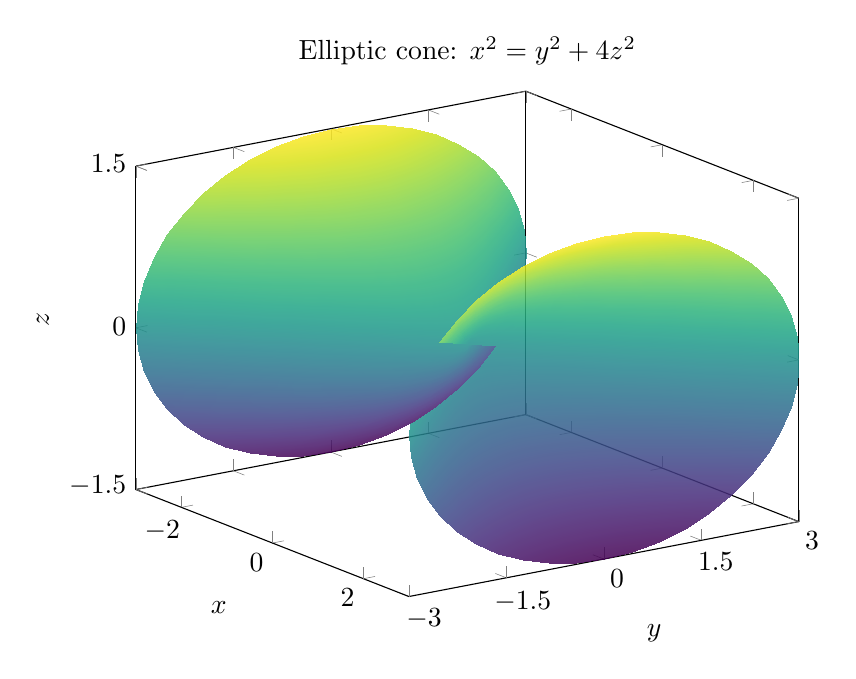
\begin{tikzpicture}
\begin{axis}[
    title={Elliptic cone: $x^2=y^2+4z^2$},
    xlabel={$x$}, ylabel={$y$}, zlabel={$z$},
    view={55}{22},
    domain=-3:3,
    y domain=0:2*pi,
    samples=45,
    samples y=45,
    colormap/viridis,
    width=10cm,
    height=8cm,
    zmin=-1.5, zmax=1.5,
    ytick={-3,-1.5,0,1.5,3},
    ztick={-1.5,0,1.5},
]
\addplot3[surf,shader=interp,opacity=0.85]
({x},{x*cos(deg(y))},{0.5*x*sin(deg(y))});
\end{axis}
\end{tikzpicture}
\end{document}